
%%%%%%%%%%%%%%%%%%%%%%%%%%%%%%%%%%%%%%%%%%%%%%%%%%%%%%%%%%%%%%%%%%%%%
%% This is a (brief) model paper using the achemso class
%% The document class accepts keyval options, which should include
%% the target journal and optionally the manuscript type.
%%%%%%%%%%%%%%%%%%%%%%%%%%%%%%%%%%%%%%%%%%%%%%%%%%%%%%%%%%%%%%%%%%%%%
\documentclass[journal=jpcbfk,manuscript=article,layout=traditional]{achemso}

%%%%%%%%%%%%%%%%%%%%%%%%%%%%%%%%%%%%%%%%%%%%%%%%%%%%%%%%%%%%%%%%%%%%%
%% Place any additional packages needed here.  Only include packages
%% which are essential, to avoid problems later.
%%%%%%%%%%%%%%%%%%%%%%%%%%%%%%%%%%%%%%%%%%%%%%%%%%%%%%%%%%%%%%%%%%%%%
\usepackage{chemformula} % Formula subscripts using \ch{}
\usepackage[T1]{fontenc} % Use modern font encodings
\usepackage{graphicx}
\usepackage{caption}
\usepackage{amsmath}
\usepackage{mathptmx}
%\usepackage[scaled=0.92]{helvet}
%%%%%%%%%%%%%%%%%%%%%%%%%%%%%%%%%%%%%%%%%%%%%%%%%%%%%%%%%%%%%%%%%%%%%
%% If issues arise when submitting your manuscript, you may want to
%% un-comment the next line.  This provides information on the
%% version of every file you have used.
%%%%%%%%%%%%%%%%%%%%%%%%%%%%%%%%%%%%%%%%%%%%%%%%%%%%%%%%%%%%%%%%%%%%%
%%\listfiles

%%%%%%%%%%%%%%%%%%%%%%%%%%%%%%%%%%%%%%%%%%%%%%%%%%%%%%%%%%%%%%%%%%%%%
%% Place any additional macros here.  Please use \newcommand* where
%% possible, and avoid layout-changing macros (which are not used
%% when typesetting).
%%%%%%%%%%%%%%%%%%%%%%%%%%%%%%%%%%%%%%%%%%%%%%%%%%%%%%%%%%%%%%%%%%%%%
\newcommand*\mycommand[1]{\texttt{\emph{#1}}}

%%%%%%%%%%%%%%%%%%%%%%%%%%%%%%%%%%%%%%%%%%%%%%%%%%%%%%%%%%%%%%%%%%%%%
%% Meta-data block
%% ---------------
%% Each author should be given as a separate \author command.
%%
%% Corresponding authors should have an e-mail given after the author
%% name as an \email command. Phone and fax numbers can be given
%% using \phone and \fax, respectively; this information is optional.
%%
%% The affiliation of authors is given after the authors; each
%% \affiliation command applies to all preceding authors not already
%% assigned an affiliation.
%%
%% The affiliation takes an option argument for the short name.  This
%% will typically be something like "University of Somewhere".
%%
%% The \altaffiliation macro should be used for new address, etc.
%% On the other hand, \alsoaffiliation is used on a per author basis
%% when authors are associated with multiple institutions.
%%%%%%%%%%%%%%%%%%%%%%%%%%%%%%%%%%%%%%%%%%%%%%%%%%%%%%%%%%%%%%%%%%%%%
\author{Sree ganesh balasubramani}
\affiliation{Department of Chemistry and Biochemistry, University of Arizona, Tucson, Arizona 85721, United States}
\author{Steven D. Schwartz}
\affiliation{Department of Chemistry and Biochemistry, University of Arizona, Tucson, Arizona 85721, United States}
%\author{I. Ken Groupleader}
%\altaffiliation{A shared footnote}
\email{sschwartz@email.arizona.edu}
%\phone{+123 (0)123 4445556}
%\fax{+123 (0)123 4445557}
%\affiliation[Unknown University]
%{Department of Chemistry, Unknown University, Unknown Town}
%\alsoaffiliation[Second University]
%{Department of Chemistry, Second University, Nearby Town}

%%%%%%%%%%%%%%%%%%%%%%%%%%%%%%%%%%%%%%%%%%%%%%%%%%%%%%%%%%%%%%%%%%%%%
%% The document title should be given as usual. Some journals require
%% a running title from the author: this should be supplied as an
%% optional argument to \title.
%%%%%%%%%%%%%%%%%%%%%%%%%%%%%%%%%%%%%%%%%%%%%%%%%%%%%%%%%%%%%%%%%%%%%
\title[]
  {Transition path sampling based calculations of free energies of enzymatic
  reactions: the case of human MAT2A and plasmodium vivax adenosine deaminase}
%%%%%%%%%%%%%%%%%%%%%%%%%%%%%%%%%%%%%%%%%%%%%%%%%%%%%%%%%%%%%%%%%%%%%
%% Some journals require a list of abbreviations or keywords to be
%% supplied. These should be set up here, and will be printed after
%% the title and author information, if needed.
%%%%%%%%%%%%%%%%%%%%%%%%%%%%%%%%%%%%%%%%%%%%%%%%%%%%%%%%%%%%%%%%%%%%%
\abbreviations{TPS,NMR,UV}
\keywords{American Chemical Society, \LaTeX}

%%%%%%%%%%%%%%%%%%%%%%%%%%%%%%%%%%%%%%%%%%%%%%%%%%%%%%%%%%%%%%%%%%%%%
%% The manuscript does not need to include \maketitle, which is
%% executed automatically.
%%%%%%%%%%%%%%%%%%%%%%%%%%%%%%%%%%%%%%%%%%%%%%%%%%%%%%%%%%%%%%%%%%%%%
\begin{document}

%%%%%%%%%%%%%%%%%%%%%%%%%%%%%%%%%%%%%%%%%%%%%%%%%%%%%%%%%%%%%%%%%%%%%
%% The "tocentry" environment can be used to create an entry for the
%% graphical table of contents. It is given here as some journals
%% require that it is printed as part of the abstract page. It will
%% be automatically moved as appropriate.
%%%%%%%%%%%%%%%%%%%%%%%%%%%%%%%%%%%%%%%%%%%%%%%%%%%%%%%%%%%%%%%%%%%%%
%\begin{tocentry}

%Some journals require a graphical entry for the Table of Contents.
%This should be laid out ``print ready'' so that the sizing of the
%text is correct.

%Inside the \texttt{tocentry} environment, the font used is Helvetica
%8\,pt, as required by \emph{Journal of the American Chemical
%Society}.

%The surrounding frame is 9\,cm by 3.5\,cm, which is the maximum
%permitted for  \emph{Journal of the American Chemical Society}
%graphical table of content entries. The box will not resize if the
%content is too big: instead it will overflow the edge of the box.

%This box and the associated title will always be printed on a
%separate page at the end of the document.

%\end{tocentry}

%%%%%%%%%%%%%%%%%%%%%%%%%%%%%%%%%%%%%%%%%%%%%%%%%%%%%%%%%%%%%%%%%%%%%
%% The abstract environment will automatically gobble the contents
%% if an abstract is not used by the target journal.
%%%%%%%%%%%%%%%%%%%%%%%%%%%%%%%%%%%%%%%%%%%%%%%%%%%%%%%%%%%%%%%%%%%%%
\begin{abstract}
  Transition path sampling (TPS) has been widely applied for the
  calculations of reaction rate, transition state and reaction 
  coordinates of condensed phase systems. Here, we discuss a scheme 
  for the calculation of free energies with the TPS method in combination 
  with a window based sampling technique. This 
  distribution can then be used for the calculations of free energies
  using standard Boltzmann inversion schemes. We calculate the free
  energy profiles of the reactions catalyzed by the human methionine 
  S-adenosyltransferase (MAT2A) enzyme and the plasmodium 
  vivax adenosine deaminase enzyme to demonstrate the applicability of this 
  method. 
\end{abstract}
%%%%%%%%%%%%%%%%%%%%%%%%%%%%%%%%%%%%%%%%%%%%%%%%%%%%%%%%%%%%%%%%%%%%%
%% Start the main part of the manuscript here.
%%%%%%%%%%%%%%%%%%%%%%%%%%%%%%%%%%%%%%%%%%%%%%%%%%%%%%%%%%%%%%%%%%%%%
\section{Introduction}
Molecular dynamics (MD) simulations are increasingly being
used to calculate quantitative estimations of experimentally measurable 
kinetic and thermodynamic parameters of enzyme catalyzed reactions. 
\cite{Karplus02NatStructMolBiol9p646,
Schramm98AnnuRevBiochem67p693,Zhang05AccChemRes38p379,
Schramm11AnnuRevBiochem80p703,Schramm18ChemRev118p11194} 
This has helped in proposing mechanisms and explanations for 
enzyme activity, fast high throughput screening of thousands of inhibitor 
molecues in drug lead discovery, \cite{Jorgensen09AccChemRes42p724,Sliwoski14PharmacolRev66p334} 
directed evolution for designing enzymes with enhanced catalytic 
activities, \cite{Thyme09Nature461p1300,Bloom09PNAS106p9995,Schafer19JAmChemSoc141p10431} etc.    
Straightforward MD simulations adequately sample 
the long-lived stable reactant and product states 
but the high energy barrier-crossing events that occur rarely and at long 
time scales are not easily accessible using this method alone.
To access such states at a higher frequency using MD simulations 
several enhanced sampling techniques 
have been developed in the past few decades some of which are 
umbrella sampling, \cite{Kastner11WileyInterdiscipRevComputMolSci1p932} 
metadynamics, \cite{Barducci11WileyInterdiscipRevComputMolSci1p826}
steered MD, \cite{Park04JChemPhys120p5946}
milestoning, \cite{Faradjian04JChemPhys120p10880} and transition path sampling 
(TPS). \cite{Pratt86JChemPhys85p5045,Bolhuis02AnnRevPhysChem53p291,Dellago98JChemPhys108p1964}

TPS in particular is an attractive method since it samples reactive trajectories
in which the rare barrier-crossing events are guaranteed to occur and
it does not require a priori knowledge of the reaction coordinate which can be 
complex for large biological systems.
TPS is based on the Monte Carlo importance sampling in the 
space of trajectories. It uses the shooting and shifting algorithm 
to collect an ensemble of reactive pathways that are real dynamical 
trajectories generated without the application of any bias forces. \cite{dellago02AdvChemPhys123} 
Therefore the TPS ensemble can be used to obtain 
kinetic information such as the rate of the reaction as well as to elucidate 
the transition state, reaction coordinate and the reaction mechanism. 
TPS has been successfully applied to study problems such as enzyme catalysis, 
\cite{Antoniou01JPhysChemB105p5553,Hay12NatChem4p161,Schwartz09NatChemBiol5p551} 
protein folding, \cite{Bolhuis03ProcNatlAcadSci100p12129,Juraszek12ChemPhys396p30} etc. 

Calculating equilibrium properties such as the free energy of an enzymatic 
catalysis reaction within TPS is not straighforward. 
The Monte Carlo algorithm used in TPS has an acceptance criterion that 
is only satisfied if the trajectory begins in the reactant basin and ends in 
the product basin or vice versa, hence trajectories that are localized in the 
reactant or product basins are rejected. The localized trajectories contribute
to the probability density distribution function ($P(\lambda)$) which is the 
probability of a system at equilibrium to have a particular value of the 
order parameter $\lambda$. \cite{Dellago09AdvCompSimAppp167} 

Frenkel has shown that inclusion of rejected states in Markov state Monte 
Carlo algorith can help speed up the convergence of the calculations of 
order-parameter distribution of a two-dimensional
Ising model. \cite{Frenkel04ProcNatAcadSci101p17571}
Inclusion of rejected trajectories within TPS was first discussed by Radhakrishnan 
et al. \cite{Radhakrishnan04JChemPhys121p2436} who developed `BOLAS' which combines 
the shooting and shifting algorithms of TPS with a window based sampling technique 
in the spirit of umbrella sampling to calculate equilibrium free energy 
differences. Peters et al. used a variant of the BOLAS scheme called the 
equilibrium path sampling (EPS) where they use aimless shooting 
combined with window based sampling for free energy calculations. 
\cite{Peters08JAmChemSoc130p17342,Beckham10epsbook} 
More recently Brotzakis et al., \cite{Brotzakis19JChemPhys151p174111}
have developed a reweighted path ensemble scheme within the standard TPS method 
called virtual interface exchange TPS (VIE-TPS) to calculate the free energy 
landscape. VIE-TPS is shown to produce reasonable free energies for 
diffusive reactions whereas it is less accurate otherwise.

Free energy calculations based on the TPS shooting algorithm is 
appealing but not a lot of examples exist in the literature 
which compare the computational calculations with experimental
results for enzymatic reactions.  
In this manuscript we implement and apply the 
algorithm developed by Radhakrishnan et al. \cite{Radhakrishnan04JChemPhys121p2436} 
to calculate the free energies of reactions catalyzed by two systems:
the human MAT2A enzyme and the plasmodium vivax adenosine deaminase 
enzyme. \cite{Luo07JAmChemSoc129p8008,Ho09Biochemistry48p9618}
These enzymes were chosen not only because of their importance in various 
biochemical applications but also because of the availability of experimental 
results with which comparisons can be drawn. The manuscript is organized as 
follows: first we discuss the TPS method and the algorithm that we use 
to calculate the free energies briefly, then we show calculations which apply this 
method on the two enzymatic reactions. Finally we compare our results to expeiments
and provide conclusions. 
%------------------------------------------------------------------------------ 
\section{Methods}
%------------------------------------------------------------------------------ 
\subsection{Transition path sampling}
%------------------------------------------------------------------------------ 
Here we briefly describe the equations describing the TPS method for the purpose of
introducing notations as well as for the sake of being complete. 
Consider the molecular dynamics simulation of a molecular system consisting 
of $N$ atoms. Starting from the initial positions and momenta of each atom at time $t_0$,
the time evolution is carried out by finding the position ($\textbf{q}$) and 
momenta ($\textbf{p}$) of each atom at regular intervals of time $t_i = t_0 + i\Delta t$  
($i = 0,1,2,\ldots$). At each of the time slices, the positions and 
momenta can be collectively represented as
the set $z = \{\textbf{q},\textbf{p}\}$. If the MD simulation is 
run for a total 
time of $\mathcal{T}$ the number of time slices is given by 
$L = \mathcal{T}/\Delta t +1$ and for this sequence of 
times the state of the system can be represented as 
\begin{equation}
z(\mathcal{T}) = \{z_0, z_{\Delta t}, z_{2\Delta t},\ldots,z_{\mathcal{T}}\}
\end{equation}
The probability to obtain a particular sequence of states is determined by the initial 
conditions and the type of dynamics used for the time evolution. If the time evolution is 
Markovian, the probability to go from $z_{i\Delta t}$ to $z_{(i+1)\Delta t}$ depends only 
on $z_{i\Delta t}$ and not on conditions before the time $i\Delta t$ the total path probablility can 
be expressed as the product of individual probabilities $p(i\rightarrow j)$ as 
\begin{equation}
\mathcal{P}[z(\mathcal{T})] = \rho(z_0)\Pi_{i=0}^{\mathcal{T}/\Delta t-1} p(z_{i\Delta t}\rightarrow z_{(i+1)\Delta t}),
\end{equation}
where $\rho(z_0)$ is the equilibrium distribution of the initial conditions and for a canonical ensemble this can be 
expressed as 
\begin{equation}
\rho(z_0) = \exp(-\beta H(z_0))/Z
\end{equation}
where 
\begin{equation}
Z = \int dz \exp(-\beta H(z)) 
\end{equation}
is the canonical partition function. 

Within the transition path sampling, the trajectories of interest start in the reactant region of the 
phase space ($\mathcal{A}$) and end in the product region ($\mathcal{B}$). Such reactive trajectories have 
a restricted probability distribution function given by
\begin{equation}
\mathcal{P}_{\mathcal{AB}}[z_{\mathcal{T}}] = h_{\mathcal{A}}(z_0)\mathcal{P}[z(\mathcal{T})]
h_{\mathcal{B}}(z_{\mathcal{T}})/Z_{\mathcal{AB}}(\mathcal{T})\label{eqn:tpsensem}
\end{equation}
where 
\[
    h_{\mathcal{A}/\mathcal{B}}(z)= 
\begin{cases}
    1, & \text{if } z\in \mathcal{A}/\mathcal{B}\\
    0,              & \text{otherwise}
\end{cases}
\]
The set of all reactive trajectories characterized by the distribution function
given by Eq. \ref{eqn:tpsensem} is the transition path ensemble. 

\subsection{Equilibrium distribution of order parameters}
%Monte carlo methods in trajectory space the probability of a path is 
%\begin{equation}
%P(x_A)
%\end{equation}
The free energy as a function of the order parameter $\zeta$ is defined
as 
\begin{equation}
\text{A}(\zeta) = -k_{\text{B}}T\text{ln}(P(\zeta)) + C, \label{eqn:fenergy}
\end{equation}
where $P(\zeta)$ is the probability distribution of the reaction coordinate
$\zeta$ and $C$ is an arbitrary constant. At equilibrium the probability distribution of the 
reaction coordinate 
can be obtained from the distribution function for the phase space $\rho(\textbf{q})$ as
\begin{equation}
P(\zeta) = \int d\textbf{V} \rho(\textbf{q})\delta\left[\zeta-\tilde{\zeta}(\textbf{q})\right].
\end{equation}
The integration is over the entire phase space. In practice the calculation of this distribution function
often proceeds using histogram based methods where the reaction coordinate is 
divided into bins and the frequency of the occurence of the reaction coordinate within a particular window
during the course of molecular dynamics simulations is used to calculate the probability distribution. 
Since some values of the reaction coordinates particulary close to the transition state are 
rarely sampled in a conventional MD simulations, enhanced sampling techniques such as the umbrella sampling
are necessary to sample the low probability regions. TPS is designed to sample these regions in phase space 
without the application of any external bias, but the trajectories sampled with TPS are only reactive and hence
they are not distributed according to the equilibrium distribution function. 
The restriction that the pathways start from the reactant state and end in the product state can be relaxed
to obtain an ensemble of trajectories that will be distributed according to the equilibrium distribution. 
%------------------------------------------------------------------------------ 
\subsection{The algorithm}
%------------------------------------------------------------------------------ 
We follow the steps proposed by Radhakrishnan et al. \cite{Radhakrishnan04JChemPhys121p2436} 
to sample TPS trajectories within windows of the order parameter. 
\begin{itemize}
  \item An appropriate order parameter is chosen for the reaction of interest 
  that can distinguish the reactant and product states sufficiently well and the TPS ensemble is harvested 
  which consists only of reactive trajectories.
\item Divide the order parameter into windows $\{\zeta_i\}$ within which the 
order parameters are given by 
$\zeta_{i}^{min} < \zeta < \zeta_{i}^{max}$.
\item Choose a reactive trajectory $\tilde{z}(\mathcal{T})$ from the TPS ensemble as 
a guiding trajectory for the window sampling. Pick a time slice from this trajectory 
$\tilde{z}_{j\Delta t}$ such that the order parameter calculated for this time slice
$\tilde{\zeta}$ satisfies $\zeta_{i}^{min} < \tilde{\zeta} < \zeta_{i}^{max}$.
\item Using the shooting and shifting algorithm familiar from TPS simulations, \cite{dellago02AdvChemPhys123}
harvest dynamics trajectories starting from the time slice $\tilde{z}_{j\Delta t}$ of the trajectory 
  $\tilde{z}(\mathcal{T})$ and accept the new trajectory if at any time slice the calculated 
  order parameter $\hat{\zeta}$ satisfies $\zeta_{i}^{min} < \hat{\zeta} < \zeta_{i}^{max}$.
  \item Calculate the probability distribution ($P_i(\zeta)$) within the window $\zeta_{i}^{min} 
  < \zeta < \zeta_{i}^{max}$ by constructing histograms obtained from the ensemble of 
  accepted trajectories for the window $i$. 
  \item Combine the probability distributions in successive windows by adjusting the constants $C$
  such that the free energy $A$ from Eq. \ref{eqn:fenergy} is continuous. 
\end{itemize}
%------------------------------------------------------------------------------ 
\section{Computational details}
%------------------------------------------------------------------------------ 
\subsection{System preparation}
%------------------------------------------------------------------------------
We used the crystal structure of the human MAT2A enzyme 
bound to methylthioadenosine and di-imido triphosphate (PNPNP)
(protein data bank ID: 7L1A) reported by Niland 
et al. \cite{Niland21Biochem60p791} and the crystal structure of \textit{pv}ADA 
in complex with MT-coformycin (protein data bank ID: 3EWC) reported by Ho et 
al. \cite{Ho09Biochemistry48p9618} as the starting points of our two 
simulations. For calculations involving the MAT2A enzyme the substrates were modified to 
L-methionine and adenosyl triphosphate (ATP) whereas for calculations with the \textit{pv}ADA
enzyme the substrates were modified to $2^{'}-$deoxyadenosine and hydroxide ion. 
MD simulations within classical and hybrid quantum mechanics/molecular mechanics 
(QMMM) approximations were carried out using the CHARMM program 
package. \cite{Brooks83JComputChem4p187,Brooks09JComputChem30p1545} 
For the MM calculations the CHARMM36 force field \cite{Brooks09JComputChem30p1545} 
was used and for the QM calculations the approximate PM3 semiempirical 
method \cite{Repasky02JComputChem23p1601} was used. 
We solvated the two proteins using TIP3P water molecules 
in a nanodroplet sphere whose volume was fixed at $15$ {\AA}
away from the protein's surface and the total charge was neutralized 
using potassium ions. 
Both the systems were minimized with 50 steps of the
steepest descent method, followed by 2000 steps of the
adopted basis Newton-Raphson method. The minimized systems were
heated slowly to 300 K for 35 ps beginning with harmonic
constraints on all atoms except on the H atoms and the TIP3 
waters with gradual reduction of the restraint forces to 1. 
15 ps of equilibration was carried out starting with harmonic 
constraints of force constant 1 followed by 20 ps of contraint free 
equilibration to prepare the systems for TPS simulations.  
%------------------------------------------------------------------------------ 
\subsection{Transition path sampling}
%------------------------------------------------------------------------------
TPS calculations collect reactive trajectories based on the Monte Carlo algorithm 
and requires a proper definition of the reactant and product states. 

The reaction catalyzed by the human MAT2A enzyme is shown in Fig. \ref{fig:mat2a-reaction}
between adenosyl $5'$-triphosphate (ATP) and L-methionine (MET) molecules resulting in the formation of
S-adenosyl-L-methionine (SAM). SAM is an essential metabolite which is distributed to almost all 
body tissues and fluids, is an universal methyl donor and is of
fundamental importance to metabolism of compounds such as hormones, neureotransmitters, proteins, 
and nucleic acids. \cite{Friedel89Drugs38p389} The reaction was experimentally characterized by 
Firestone et al. \cite{Firestone17JAmChemSoc139p13754} to follow a S$_{\text{N}}2$ transition 
state. The key bond parameters for this reaction consists of the distance between the
nucleophilic sulfur atom of MET and the $5'-C$ atom of the ATP ($S-C$), and the distance between 
oxygen atom of the phosphate group and the $5'-C$ atom of ATP ($O-C$).
For the TPS calculations we define the reactant state to have $O-C$ distance to be 
less than 1.7 {\AA} and the product state to have the $S-C$ distance being less than 1.7 {\AA}. 

\begin{figure}

\includegraphics[scale=0.6]{figures/mat2a-reaction.png}
\caption{The reaction catalyzed by human MAT2A enzyme}
\label{fig:mat2a-reaction}
\end{figure}

The reaction catalyzed by $pv$ADA is shown in  
Fig. \ref{fig:ada-reaction} which is between the adenosine molecule and a hydroxide ion
which results in the formation of inosine with ammonia as a by product. 
$pv$ADA is an essential enzyme in the purine salvage pathway for plasmodium vivax and 
inhibiting this enzyme is a promising approach to treat malaria. \cite{Madrid08JBiolChem283p35899}  
This reaction proceeds with the nucleophilic O atom (O$^{\text{hydroxyl}}$) of the hydroxide anion
attacking the electrophilic C6 atom of the adenosyl ring leading to the formation of a Meisenheimer 
complex while the N1 atom on the adenosyl ring starts to get 
protonated by the Glu229 residue of $pv$ADA. At the transition state, experimental findings 
suggest that the dissociation of the C6$-$N6 bond as well as the protonation of the N1 
atom are almost complete. \cite{Luo07JAmChemSoc129p8008} The key bond parameters are 
the distance between the approaching hydroxyl oxygen and the C6 atom ($O-C$) and the 
dissociating C6$-$N6 ($N-C$) bond distance. For the TPS simulaions we defined the reactant state to 
have the $O-C$ distance being less than $1.7$ {\AA} and the product state to have the $O-C$ 
distance being less than $1.7$ {\AA}.

\begin{figure}

\includegraphics[scale=0.6]{figures/ada-new.png}
\caption{The reaction catalyzed by adenosine deaminase enzyme}
\label{fig:ada-reaction}
\end{figure}

A biased initial reactive trajectory is obtained by using harmonic restraint forces 
of 1500 to break the $O-C$ bond and form the $S-C$ bond for the MAT2A enzyme and 
to break the $N-C$ bond and form the $O-C$ bond for the case of the $pv$ADA enzyme. 
Using the biased trajectory as the starting point and after removing the restraint 
forces, the shooting algorithm was used to generate
new trajectories within which first a random time slice is chosen from the reactive 
trajectory and perturbing the momenta of the system. 
The time step that we used for all our calculations was $1\;fs$ and we propagate the 
dynamics for a total of 250 steps forward and 250 steps backward which amounts to a 
total of $0.5\;ps$. 
A total of 150 and 100 reactive trajectories were generated for the MAT2A and $pv$ADA
enzymes, respectively. 

%------------------------------------------------------------------------------ 
\subsection{Free energy calculations}
%------------------------------------------------------------------------------ 
Window based free energy calculations such as WHAM divide the reaction coordinate
into windows and calculate the individual populations within the windows and 
decouple the applied bias with some formulas. 
For the free energy calculations we divided the reaction coordinate into 13 windows for 
MAT2A and 20 windows for pvADA with a $15\%$ overlap on each side of the window. 

%------------------------------------------------------------------------------ 
\section{Results and discussion}
%------------------------------------------------------------------------------ 
\subsection{Human Methionine Adenosyltransferase 2A}
%------------------------------------------------------------------------------ 
Human methionine adenosyltransferase (MAT2A) is an enzyme that catalyzes the 
reaction between adenosine triphosphaste and L-methionine which leads to the 
formation of S-Adenosylmethionine. \cite{Firestone17JAmChemSoc139p13754,Niland21Biochem60p791} 
The mechanism of this reaction is experimentally determined to follow a 
SN$_2$ transition state with the sulphur atom of the L-methionine as the 
nucleophile with the triphosphate leaving group.  

\begin{figure}[ht!]
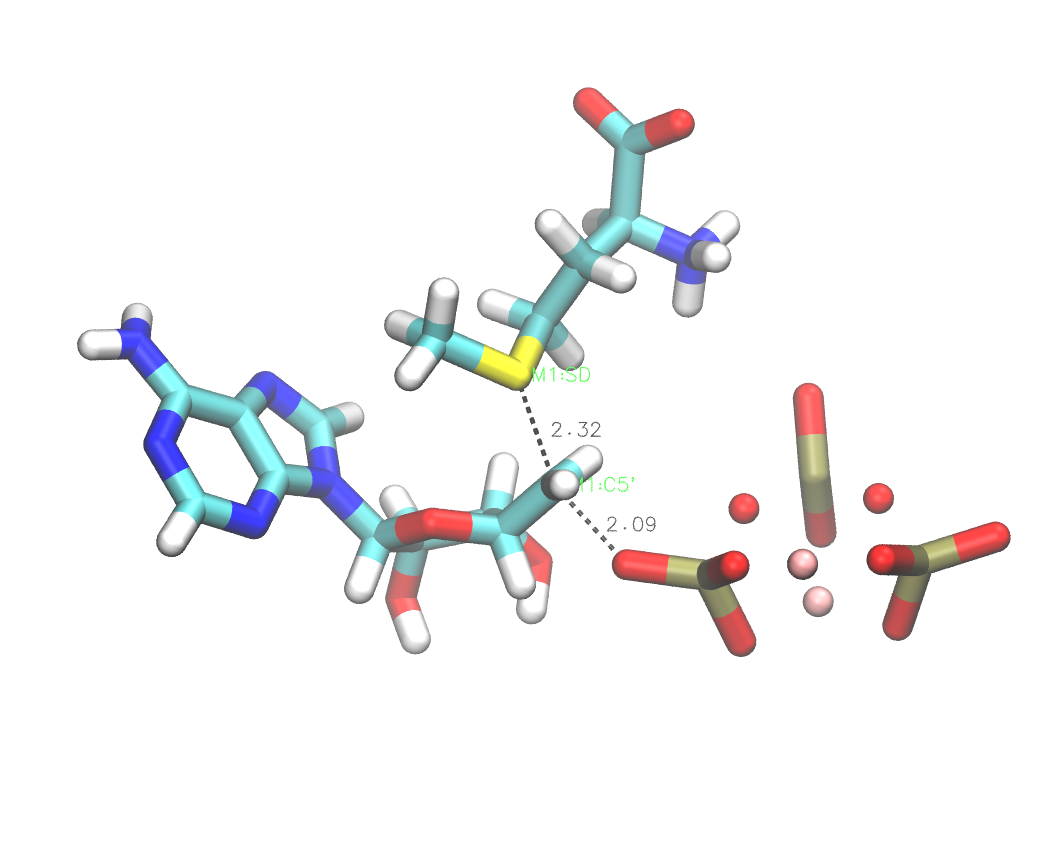
\includegraphics[scale=0.25]{figures/mat2a-transition-state.png}
\end{figure}

\begin{figure}[ht!]
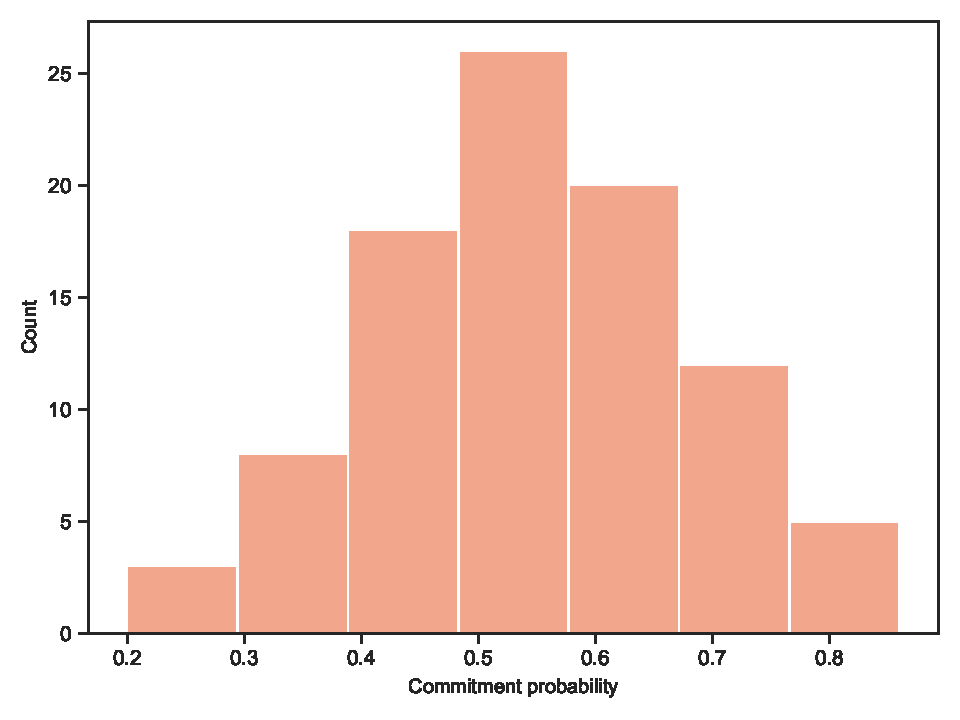
\includegraphics[scale=0.5]{figures/comm-60-mat2a.pdf}
\end{figure}

\begin{figure}
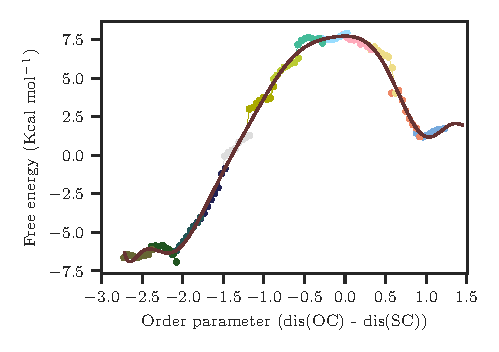
\includegraphics[scale=0.5]{figures/mat2a-fenergy.pdf}
\caption{The free energy as a function of the order parameter.}
\end{figure}

%------------------------------------------------------------------------------ 
\subsection{Adenosine deaminase reaction coordinates and free energy}
%------------------------------------------------------------------------------ 
\begin{figure}[ht!]
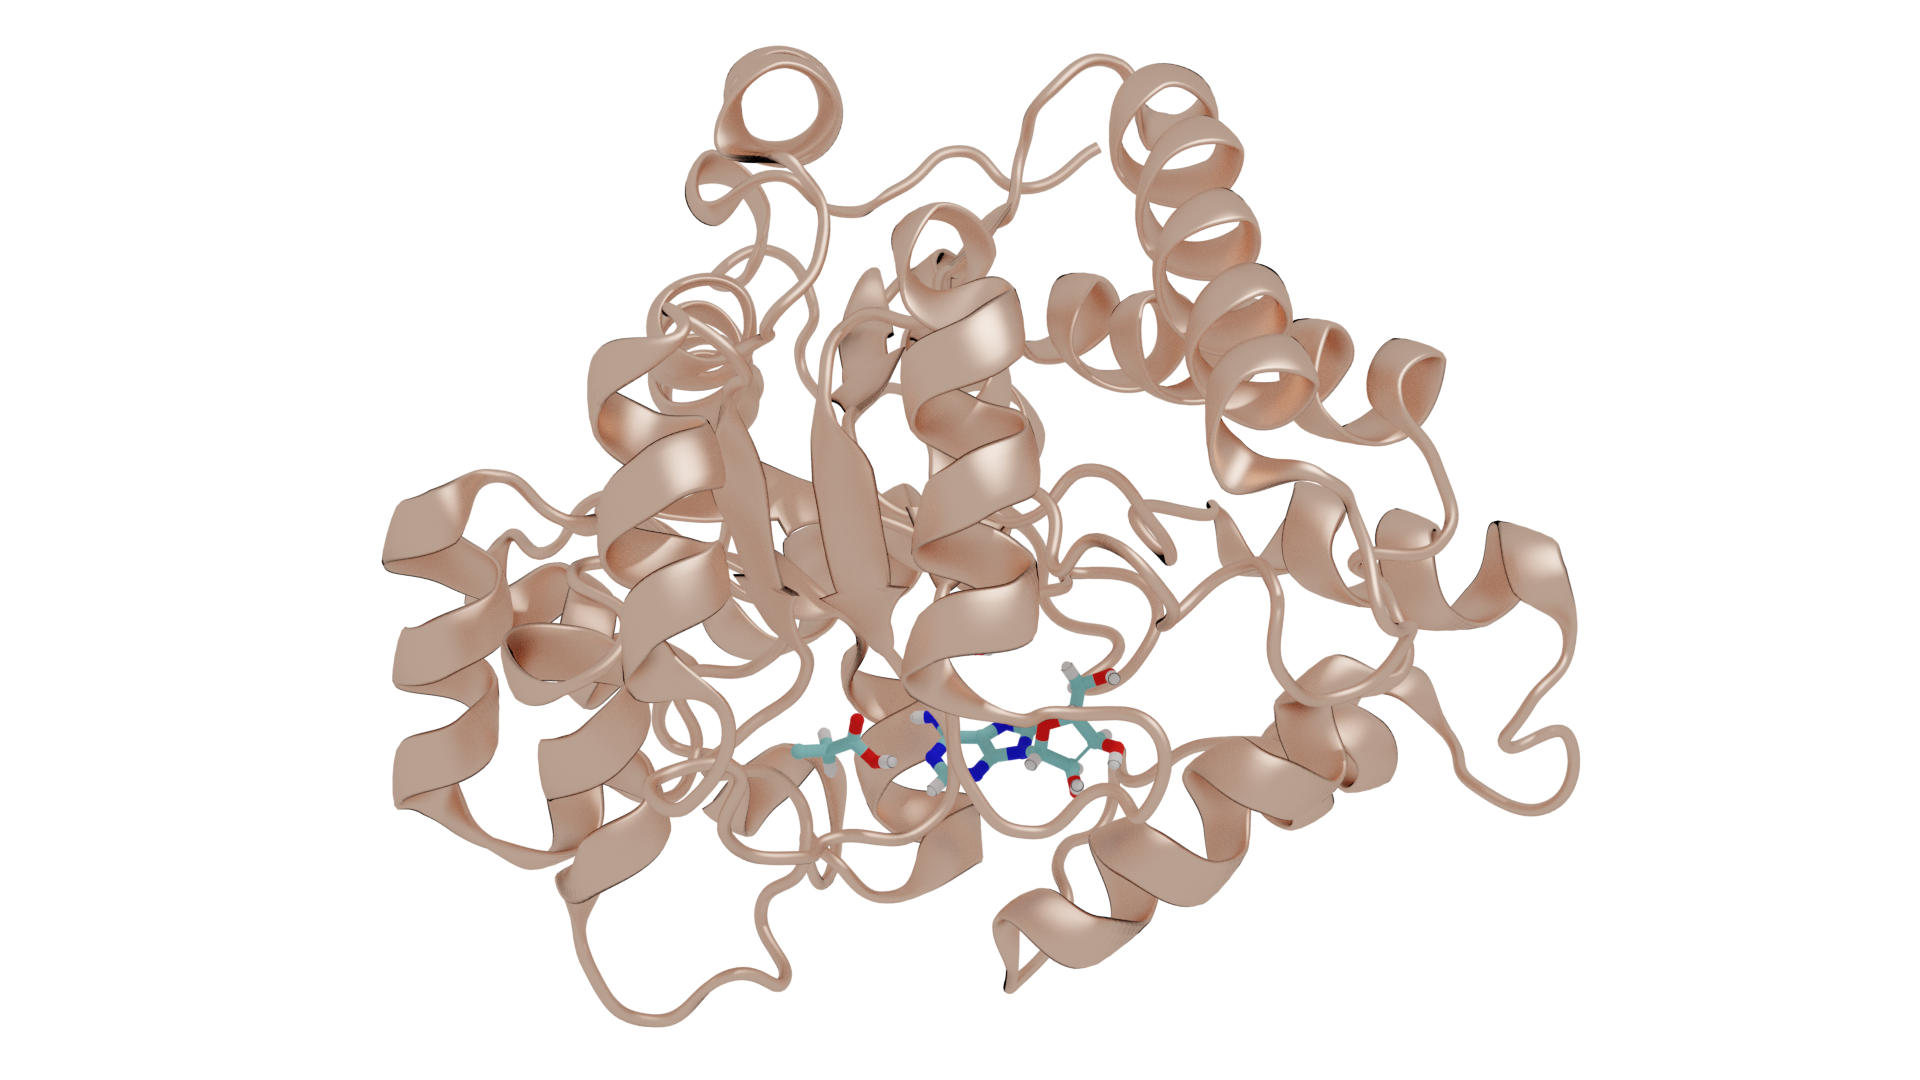
\includegraphics[scale=0.15]{./figures/ada-protein.png}
\end{figure}

\begin{figure}[ht!]
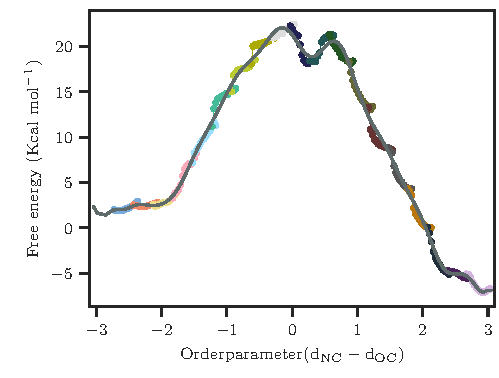
\includegraphics[scale=0.5]{./figures/ada-fenergy.pdf}
\end{figure}

%\begin{figure}[ht]
%\centering
%\begin{minipage}[b]{0.32\linewidth}
%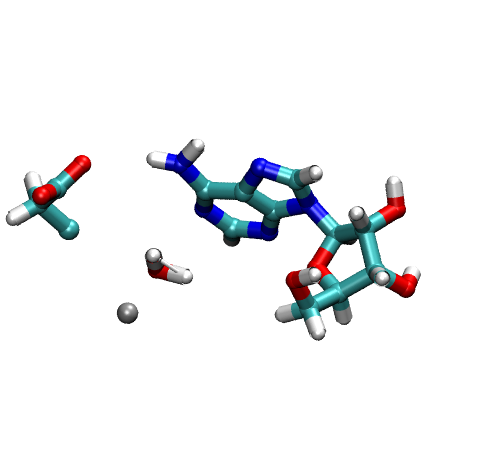
\includegraphics[scale=0.3]{figures/reactant-state.png}
%\caption{Reactant state}
%\label{fig:minipage1}
%\end{minipage}
%\quad
%\begin{minipage}[b]{0.32\linewidth}
%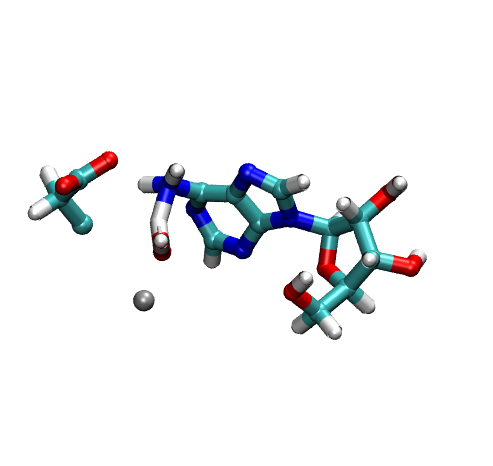
\includegraphics[scale=0.3]{figures/int1.png}
%\caption{Intermediate state}
%\label{fig:minipage2}
%\end{minipage}
%\quad
%\begin{minipage}[b]{0.32\linewidth}
%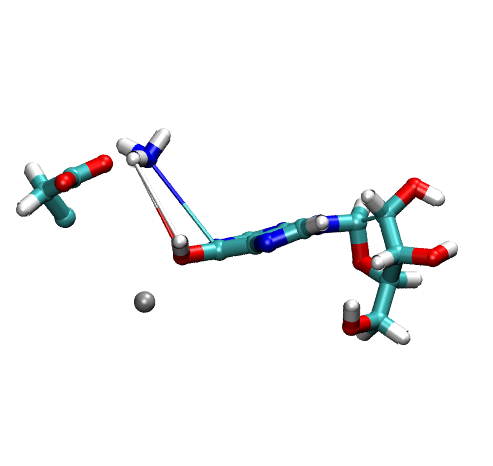
\includegraphics[scale=0.3]{figures/product-state.png}
%\caption{Product state}
%\label{fig:minipage1}
%\end{minipage}
%\end{figure}
%------------------------------------------------------------------------------ 
\section{Conclusions}
%------------------------------------------------------------------------------ 
We have discussed the application of a scheme to calculate the 
free energies of enzymatic reactions within the TPS method using the MAT2A
and the ADA enzymes as examples. 

%%%%%%%%%%%%%%%%%%%%%%%%%%%%%%%%%%%%%%%%%%%%%%%%%%%%%%%%%%%%%%%%%%%%%
%% The "Acknowledgement" section can be given in all manuscript
%% classes.  This should be given within the "acknowledgement"
%% environment, which will make the correct section or running title.
%%%%%%%%%%%%%%%%%%%%%%%%%%%%%%%%%%%%%%%%%%%%%%%%%%%%%%%%%%%%%%%%%%%%%
\begin{acknowledgement}


\end{acknowledgement}

%%%%%%%%%%%%%%%%%%%%%%%%%%%%%%%%%%%%%%%%%%%%%%%%%%%%%%%%%%%%%%%%%%%%%
%% The same is true for Supporting Information, which should use the
%% suppinfo environment.
%%%%%%%%%%%%%%%%%%%%%%%%%%%%%%%%%%%%%%%%%%%%%%%%%%%%%%%%%%%%%%%%%%%%%
\begin{suppinfo}


\end{suppinfo}

%%%%%%%%%%%%%%%%%%%%%%%%%%%%%%%%%%%%%%%%%%%%%%%%%%%%%%%%%%%%%%%%%%%%%
%% The appropriate \bibliography command should be placed here.
%% Notice that the class file automatically sets \bibliographystyle
%% and also names the section correctly.
%%%%%%%%%%%%%%%%%%%%%%%%%%%%%%%%%%%%%%%%%%%%%%%%%%%%%%%%%%%%%%%%%%%%%
\bibliography{manuscript}

\end{document}
